\section{Background}
\label{background}
This section will present relevant background information for reading this paper, including the research area in section \ref{research_area}, the \qs{} algorithm in \ref{qs}, and related work in \ref{state_of_the_art}.

\subsection{Research area}
\label{research_area}
%What is the research area?
Various algorithms exist to find distances between data points in a (typically large) data set. One example is doing similarity search, or more specifically ANN search, on pictures to recognize letters or numbers. As useful as this is, it still depends on the given data, which is getting increasingly big in size and suffers from the \textit{curse of dimensionality}. This is a general problem as even modern machines are not able to process \textit{gigantic} files all at once(i.e. keeping all the data in main memory). Thus another big subject in computer science arises, that is compressing the data in order to fit it in memory while trying to preserve relevant properties from the data. One particular scheme is referred to as \textit{quantization}, which is the process of constraining an input from a continuous set of values to a discrete set\footnote{E.g. real numbers to integers. See https://en.wikipedia.org/wiki/Quantization 11-04-2018}. This research area is what \qs{} deals with, and in particular for high-dimensional data sets. 
\\
\\
Naturally one must pay to compress something, which happens in terms of accuracy, i.e. representing the data using only approximations. This also means there is a trade off between compression and accuracy for the algorithms in this area. Compression algorithms are usually measured on these parameters, i.e. accuracy per compression size\cite{wagner17,schmid9}.
\\
\\
Distance preserving compression algorithms are usually divided into two categories: data-oblivious and data-dependent. The former attempts to achieve guarantees for any data set while the latter attempts to use the extra information about the particular data sets in order to design functions with better performance. Compressed representations makes computation for data analysis algorithms more efficient, which is very desirable in many fields, such as data mining and machine learning\cite{stan15}.

\subsection{The \qs{} compression scheme}
\label{qs}
In this section the \qs{} algorithm is outlined. The compression scheme that it comprises produces a sketch, which is a compressed representation of a point set \texttt{X}. The points of \texttt{X} have \texttt{d} dimensions and are in \textit{Euclidean} space. Each coordinate of a point is represented by \texttt{B} bits implying that a point is represented by \textit{dB} bits. \qs{} requires the point set \texttt{X} and two additional parameters, namely \texttt{L} and $\Lambda$ as input. These two parameters are used to specify the compression of the point set where \texttt{L} is the depth of the \qt{} and $\Lambda$ controls the amount of nodes from \qt{} which can be pruned. Furthermore a number of \textit{blocks} is required to run the extended algorithm presented in \tm{3}(see below).

There are three steps for building the sketch: randomly shifted grid, \qt{} construction and pruning. These steps will be explained briefly and a small example of how a \qt{} is built and pruned will be given.
\\
\\
The first step is to produce a randomly shifted grid on the hypercube(an n-dimensional space) \texttt{H} which contains all points of the given point set \texttt{X}. \texttt{H} will then be set up to be centered around a point of \texttt{X}. Then a random value, $\sigma_j$, is chosen for each dimension \texttt{j} to shift \texttt{H}. This results in a randomly shifted axis-parallel grid on the points. It is however noted in the paper that this step often can be eliminated in practice without affecting the empirical performance of the algorithm, but that it is necessary for achieving guarantees for arbitrary point sets\cite[p. 4, "Step 1"]{wagner17}.
\\
\\
The next step is to create the \qt{}. A \qt{} is created by starting at the root of \texttt{H}. Child nodes are only added for the corresponding grid cells that contain at least one point of \texttt{X}, and thus child nodes that do not contain a point from \texttt{X} are ignored. Each edge to a child node is labeled with a \textit{d} long bit string that represents the values split on for each dimension. This step is done recursively until the level \textit{L} is reached. An example of a constructed \qt{} is given in figure \ref{fig:quadtree}(on the left).\\

\begin{figure}
	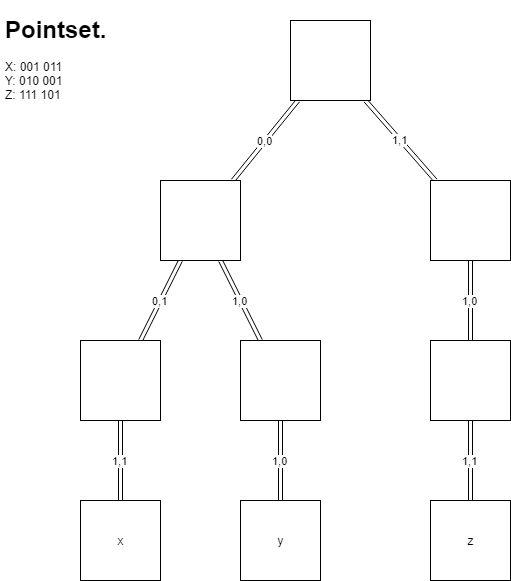
\includegraphics[width=0.5\textwidth]{figures/quadtree}
	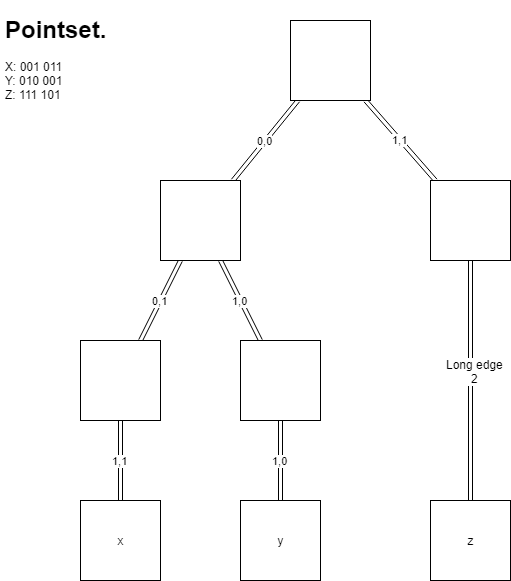
\includegraphics[width=0.5\textwidth]{figures/prunnedquadtree}
	\caption{On the left there is shown the \qt{} after construction with $L=4$. On the right the \qt{} has been pruned with a $\Lambda = 1$}
	\label{fig:quadtree}
\end{figure}

The final step is pruning. For each downward path $n_0,...,n_k$ in the \qt{} where nodes $n_1,...,n_{k-1}$ all have a degree 1, if \ensuremath{\texttt{k} > \Lambda+1} then corresponding nodes $n_{\Lambda+1},...,n_{k-1}$ are removed from the \qt{}. Instead node $n_{\Lambda}$ is connected directly to $n_{k}$ with an edge. This edge is called a \textit{long edge} and is labeled with the length of the path it replaces ($k-\Lambda$). An example of the tree after a pruning is given in figure \ref{fig:quadtree}(on the right).
\\
\\
To represent the sketch the "Eulerian Tour Technique"\footnote{See e.g., \url{https://en.wikipedia.org/wiki/Euler\_tour\_technique}} is used.
It starts at the root of the tree and searches down to the leftmost leaf. It will then backtrack up to a node from which it came and traverse down to find a new leaf in a depth first search manner. When an edge is explored downwards a 0 is stored together with the label of the edge, being either a bit string or the length of a long edge and a bit specifying if the given edge is a long or short edge. If an upwards edge is explored a 1 is stored. Furthermore an index for all the leafs are stored.
\\
\\
The paper \cite{wagner17} present three different approaches for building the previous described sketch each giving different properties for the resulting sketch. These different properties are defined as theorems, \tm{1} being the primary theorem.

\paragraph{\tm{1}} states that for each point, the distance from the given point to all other points are preserved up to a given factor $1\pm\epsilon$ with a constant probability. This is formalized as the following guarantee: for every $i\in{[n]}$
\begin{equation}
Pr[\forall{}_{j\in{}[n]} ||~x_i-~x_j||= (1\pm\epsilon)||x_i-x_j||] \geq 1 - \delta
\end{equation}
\paragraph{\tm{2}} states the property of being able to recover \textit{every} distance $||x_i-x_j||$  up to a distortion $1\pm\epsilon$ with a high probability by applying \qs{} recursively.
\paragraph{\tm{3}} is an extension of \tm{1} in which a sketch is built for $m$ blocks where a block is a subset of dimensions for the points in the dataset $X$. Here \qs{} is applied separately to each block. This gives the following guarantee, with \textit{m} added:

\begin{equation}
Pr[\forall{}_{j\in{}[n]} ||~x_i-~x_j||= (1\pm\epsilon)||x_i-x_j||] \geq 1 - m\delta
\end{equation}

%From ILO:
%"Find, extract and explain results in the algorithms research literature relevant to a given problem."
\subsection{Related work}
\label{state_of_the_art}
Due to the size of the research area, described in \ref{research_area}, a huge amount of related work to \qs{} exists. \cite{wagner17} specifically compares their algorithm to a state of the art algorithm, \textit{Product Quantization} (\pq{}), introduced in \cite{schmid9}. %Furthermore Spectral Hashing is closely relates as... Also the findings in [6] shows that...
%TODO: Write which papers are related

\subsubsection{\textit{Product Quantization}}
The \pq{} concept is stated in the abstract of the original paper as such: \textit{This paper introduces a product quantization based approach for approximate nearest neighbor search. The idea is to decompose}[..] \textit{the space into a Cartesian product of low dimensional subspaces and to quantize each subspace separately}. Specifically the algorithm uses \textit{vector quantization} as the approach to compress data, mapping a real valued vector, \textit{x}, in \textit{D}-dimensional space to \textit{centroid} representations, \textit{$c_i$}, in a set $\mathcal{V}_i$\cite[p.3 II-A]{schmid9}. The set of vectors mapped with the quantizer function \textit{q} to a given index \textit{i} is referred to as a (Voronoi) \textit{cell}, and defined as:

\begin{equation}
	\mathcal{V}_i\mathrel{\hat=}{x\in\mathbb{R}^D : q(x)=c_i}
\end{equation}

As opposed to scalar quantization, where single values are reconstructed, in this case the set of \textit{vectors}, indexed to the same cell, are reconstructed. Before applying this scheme to the vectors, the D dimensions are divided into \textit{product quantizers}, basically dividing the space into \textit{m} subvectors of \textit{D*} dimensions, such that \textit{D*$=D/m$}\cite[p.3 II-B]{schmid9}. The subvectors are then quantized seperately using \textit{m} distinct quantizers. This scheme is applied, allowing to keep very large vector codes in memory. As reference a convincing example is listed in \cite[Table I, p. 4]{schmid9}, illustrating that the k-means algorithm consumes $kD$ memory, while k-means with product quantization consumes  $k^{1/m}D$.

Besides using \pq{} as comparison algorithm in their experiments, \qs{} is actually implemented with the same idea of \textit{product quantizers}\footnote{specifically defined in \tm{3}, \cite[p. 5]{wagner17}}. \qs{} is applied to all data points for each subvector in \textit{D*} dimensions, which is referred to as \textit{blocks} in their paper. 

\subsubsection{Hashing methods} %TODO: Cite
Further algorithms on data-dependent distance preserving compression algorithms include Locality Sensitive Hashing(LSH), Semantic Hashing, and Spectral Hashing\cite{weiss8}, which all rely on hash functions for computing codes. 

The former algorithm, LSH, is popular, and widely used as reference in the research area. Instead of using a tree-like data structure, such as a kd-tree, it hashes points using several hash functions, ensuring that, for each function, the probability of collision is much higher for objects which are close to each other than for those that are far apart\footnote{It is worth noting that this is the exact opposite of what is trying to be achieved in e.g. hash tables}. Thus, one can use this scheme to hash a query point, and then retrieve near neighbors contained in the same hash bucket.

Semantic Hashing computes compact codes for data points such that the Hamming distance between two different codes are correlated with \textit{semantic similarity}(i.e. the idea of distance is based on the likeness of meaning or semantic content\footnote{\url{https://en.wikipedia.org/wiki/Semantic_similarity}. Accessed 14-05-2018}). Similar neighbors are then computed by retrieving items within a small Hamming distance from the code of the query.  

Similarly Spectral Hashing tries to obtain binary code representation of data points. This algorithm uses a bit more complex approach. It first performs a Principal component analysis (PCA) on the data, which converts it to a \textit{set of values of linearly uncorrelated variables called principal components}\footnote{\url{https://en.wikipedia.org/wiki/Principal_component_analysis}. Accessed 14-05-2018}. Then a concept of fitting a rectangular approximation along every PCA direction is performed by finding the \textit{k} smallest eigenvalues\footnote{A vector that only changes by a scalar factor when applied with a linear transformation. \url{https://en.wikipedia.org/wiki/Eigenvalues_and_eigenvectors}. Accessed 14-05-2018.}, and finally thresholding these to obtain binary codes(i.e. setting a 1 when a value is above some threshold, otherwise 0). 

\subsubsection{Near-Optimal (Euclidean) Metric Compression}
Referenced throughout \cite{wagner17} is the paper \cite{NearO}. This paper describes a method using two collaborative algorithms to construct a sketch for \textit{n} points of size \bo{nlog(1/$\epsilon$) + log log $\Phi$}, where $\Phi$ denotes the aspect ratio(see \ref{sec:aspect_ratio}). This is a lower bound than achieved by \qs{}. This method is related to \qs{} both in research area, but also in nature of the algorithms. The algorithms are based on a hierarchical clustering of the points and both uses similar pruning techniques in order to reduce the size of sketch.
\\
\\
The method described in \cite{NearO} makes use of two algorithms, namely a \textit{summation} algorithm \texttt{SUM} and an \textit{estimation} algorithm \texttt{EST}. \texttt{SUM} makes up most of the paper as this is the algortihm responsible for constructing the sketch. The \texttt{EST} algorithm is responsible for approximating the distance between two points in the sketch.

\texttt{SUM} constructs a variant of hierarchically well-separated trees (HST's) connecting each cluster C in a dataset to its related subclusters. Every node in the tree T has a mapping to their related clusters. The tree T has \textit{n} leaves and a depth up to \textit{log $\Phi$ + 2} prior to the \textit{compression} step. This compression step is quite similar to the pruning step in \cite{wagner17}, as it compresses long paths of degree-1 nodes.
\\
\\
After the compression of T, a different approach to represent the nodes than in \cite{wagner17} is used. Instead of using quantization as with \qs{}, \cite{NearO} associates three properties for each node \textit{v} $\in$ T. Firstly it associates a center, \textit{c(v)}, secondly an ingress \textit{in(v)} and thirdly a surrogate \textit{s*(v)}. %The function \textit{c(v)} points to the node which represents the center of the cluster to which \textit{v} belongs, and \textit{s*(v)} describes the approximate location of this center from \textit{v}. The \textit{in(v)} function points to another node in the same subtree as \textit{v} and is used to calculate \textit{v's} displacement from its center. 
Once these properties have been associated to each node in T, the sketch is created, storing the nodes and the structure of T, denoting long edges and short edges similarly as in \qs{}. 
\\
\\
Once the sketch has been created the method now makes use of the \texttt{EST} algorithm to produce a (1 $\pm$ $\epsilon$)-approximation for the distance between any two points in the given dataset. \texttt{EST} is able to recover the approximate surrogates related to a point, and since the surrogates exist in the same subtree as the original point. It is hence possible to deduce the approximate distance. 
%Well known general algorithms and data structures exists for the same purpose, such as \textit{k-means} and \textit{kd-trees}, where the former is a clustering algorithm and the latter is an adaptive data structure for spatial data sets. This is also discussed in \cite{schmid9}, where it is noted that apparently a pure brute-force algorithm outperforms these in practice for high-dimensional data. Further algorithms listed in this paper include "spectral hashing"\cite{weiss8}, "Hamming embedding"\cite{jegou8}, and "FLANN"\cite{muja9}. These will not be investigated further, but are only mentioned for reference.
%TODO: Elaborate on closely related work and insert citations